\section{Produits}
\subsection{Framework RMIAGE}

\subsubsection{Côté client} % (fold)
\label{ssub:côté_client}
Les sources du client sont entièrement fournies au client pour lui permettre toute forme de modifications, notamment graphiques, liées à gestion des inscriptions ou aux informations d'identification utilisées pour la connexion.

La fenêtre de connexion permet de saisir ces informations. À la demande de connexion, un gestionnaire de réseau est créé. En cas d'échec, un message est affiché dans la fenêtre connexion.

Dans le cas contraire, le gestionnaire de réseau acquière un contrôleur de session auprès du serveur. Il initialise alors un fil d'exécution dont le rôle est de permettre au serveur de \emph{pusher} des messages à tout moment (pour les fournir au panneau par exemple) et une fenêtre principale. Cette fenêtre dispose d'éléments graphiques pour la recherche et la déconnection, pour l'instant inutilisés, d'un arbre de navigation transmis par le serveur et mis à jour sur demande du serveur. Un panneau de droite est initialisé.

À chaque déplacement dans l'arbre de navigation, le client demande au serveur le panneau correspondant (classe et données) et le substitue au panneau jusqu'ici utilisé. Le précédent panneau peut effectuer des actions avant de restituer l'emplacement.

Ces panneaux disposent d'un accès au contrôleur de session, et peuvent lui transmettre des messages.

Des fenêtres de \emph{popup} sont disponibles, et utilisables directement par le serveur grâce à un type de message spécifique.
% subsubsection côté_client (end)

\subsubsection{Côté serveur} % (fold)
\label{ssub:côté_serveur}

\begin{figure}[thbp]
	\centering
		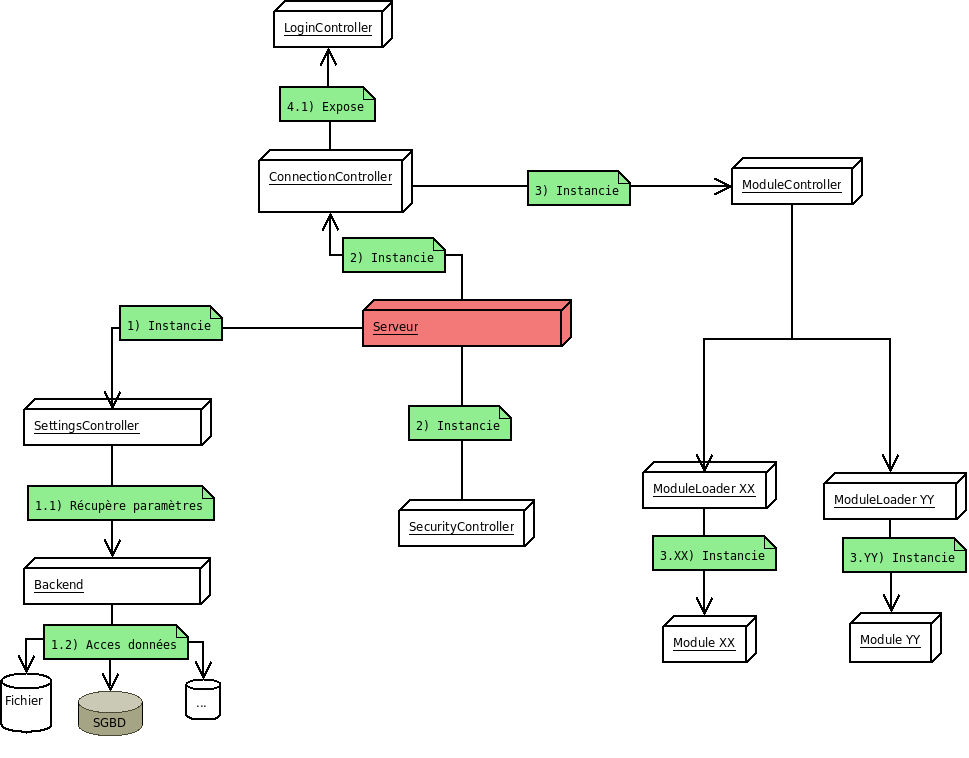
\includegraphics[angle=90,scale=0.6]{../diagrammes/init_server.png}
	\caption{Scénario d'initialisation du serveur}
	\label{fig:init_server}
\end{figure}

\begin{figure}[thbp]
	\centering
		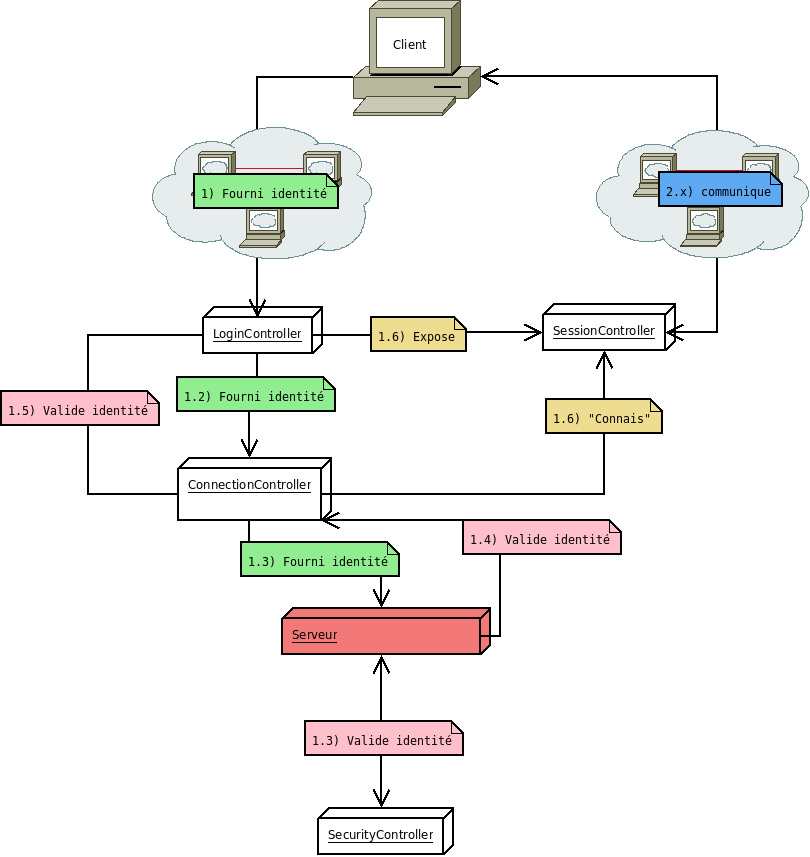
\includegraphics[scale=0.6]{../diagrammes/auth_client.png}
	\caption{Scénario d'authentification d'un client}
	\label{fig:auth_client}
\end{figure}

Le serveur, controlleur principal, quand à lui consiste en une application "glue" des différents composants du framework développé.

La configuration de cette application se fait via un gestionnaire de configuration, étendable par notre client à son grés.


Ce gestionnaire de configuration sert dans un premier temps à instancier un controleur implémentant la couche réseau, ici le protocole RMI :
Ce "NetworkController" peut récupérer à partir du controllleur principal deux paramètre nécessaires à son fonctionnement :
\begin{itemize}
 \item le nom de la ressource principale à exposer (adresse à laquelle le serveur est joignable)~;
 \item une instance de l'objet principal à exposer.
\end{itemize}
De même, il initialise un contolleur de module, chargé d'initialiser les différents modules via les chargeurs de modules paramétrés, récupérés via le gestionnaire de configuration.

Dans notre cas, l'objet principal est un "LoginController", permettant d'initialiser une nouvelle session avec le client si les informations fournies par le client sont validées par le gestionnaire d'identification, et retourne alors un controlleur de session permettant d'effectuer de faire appel 


Le détail du scénario de l'initialisation du serveur est donnée fig.\ref{fig:init_server}, p.\pageref{fig:init_server}.

De même, à titre d'exemple, le scénario de l'authentification d'un client est donné fig.\ref{fig:auth_client}, p.\pageref{fig:auth_client}. Note : le gestionnaire de session crée permet la communication avec les modules via le gestionnaire de connection. Cette partie est volontairement omise pour alléger le client.
% subsubsection côté_serveur (end)